\subsection{Sequence Diagram}
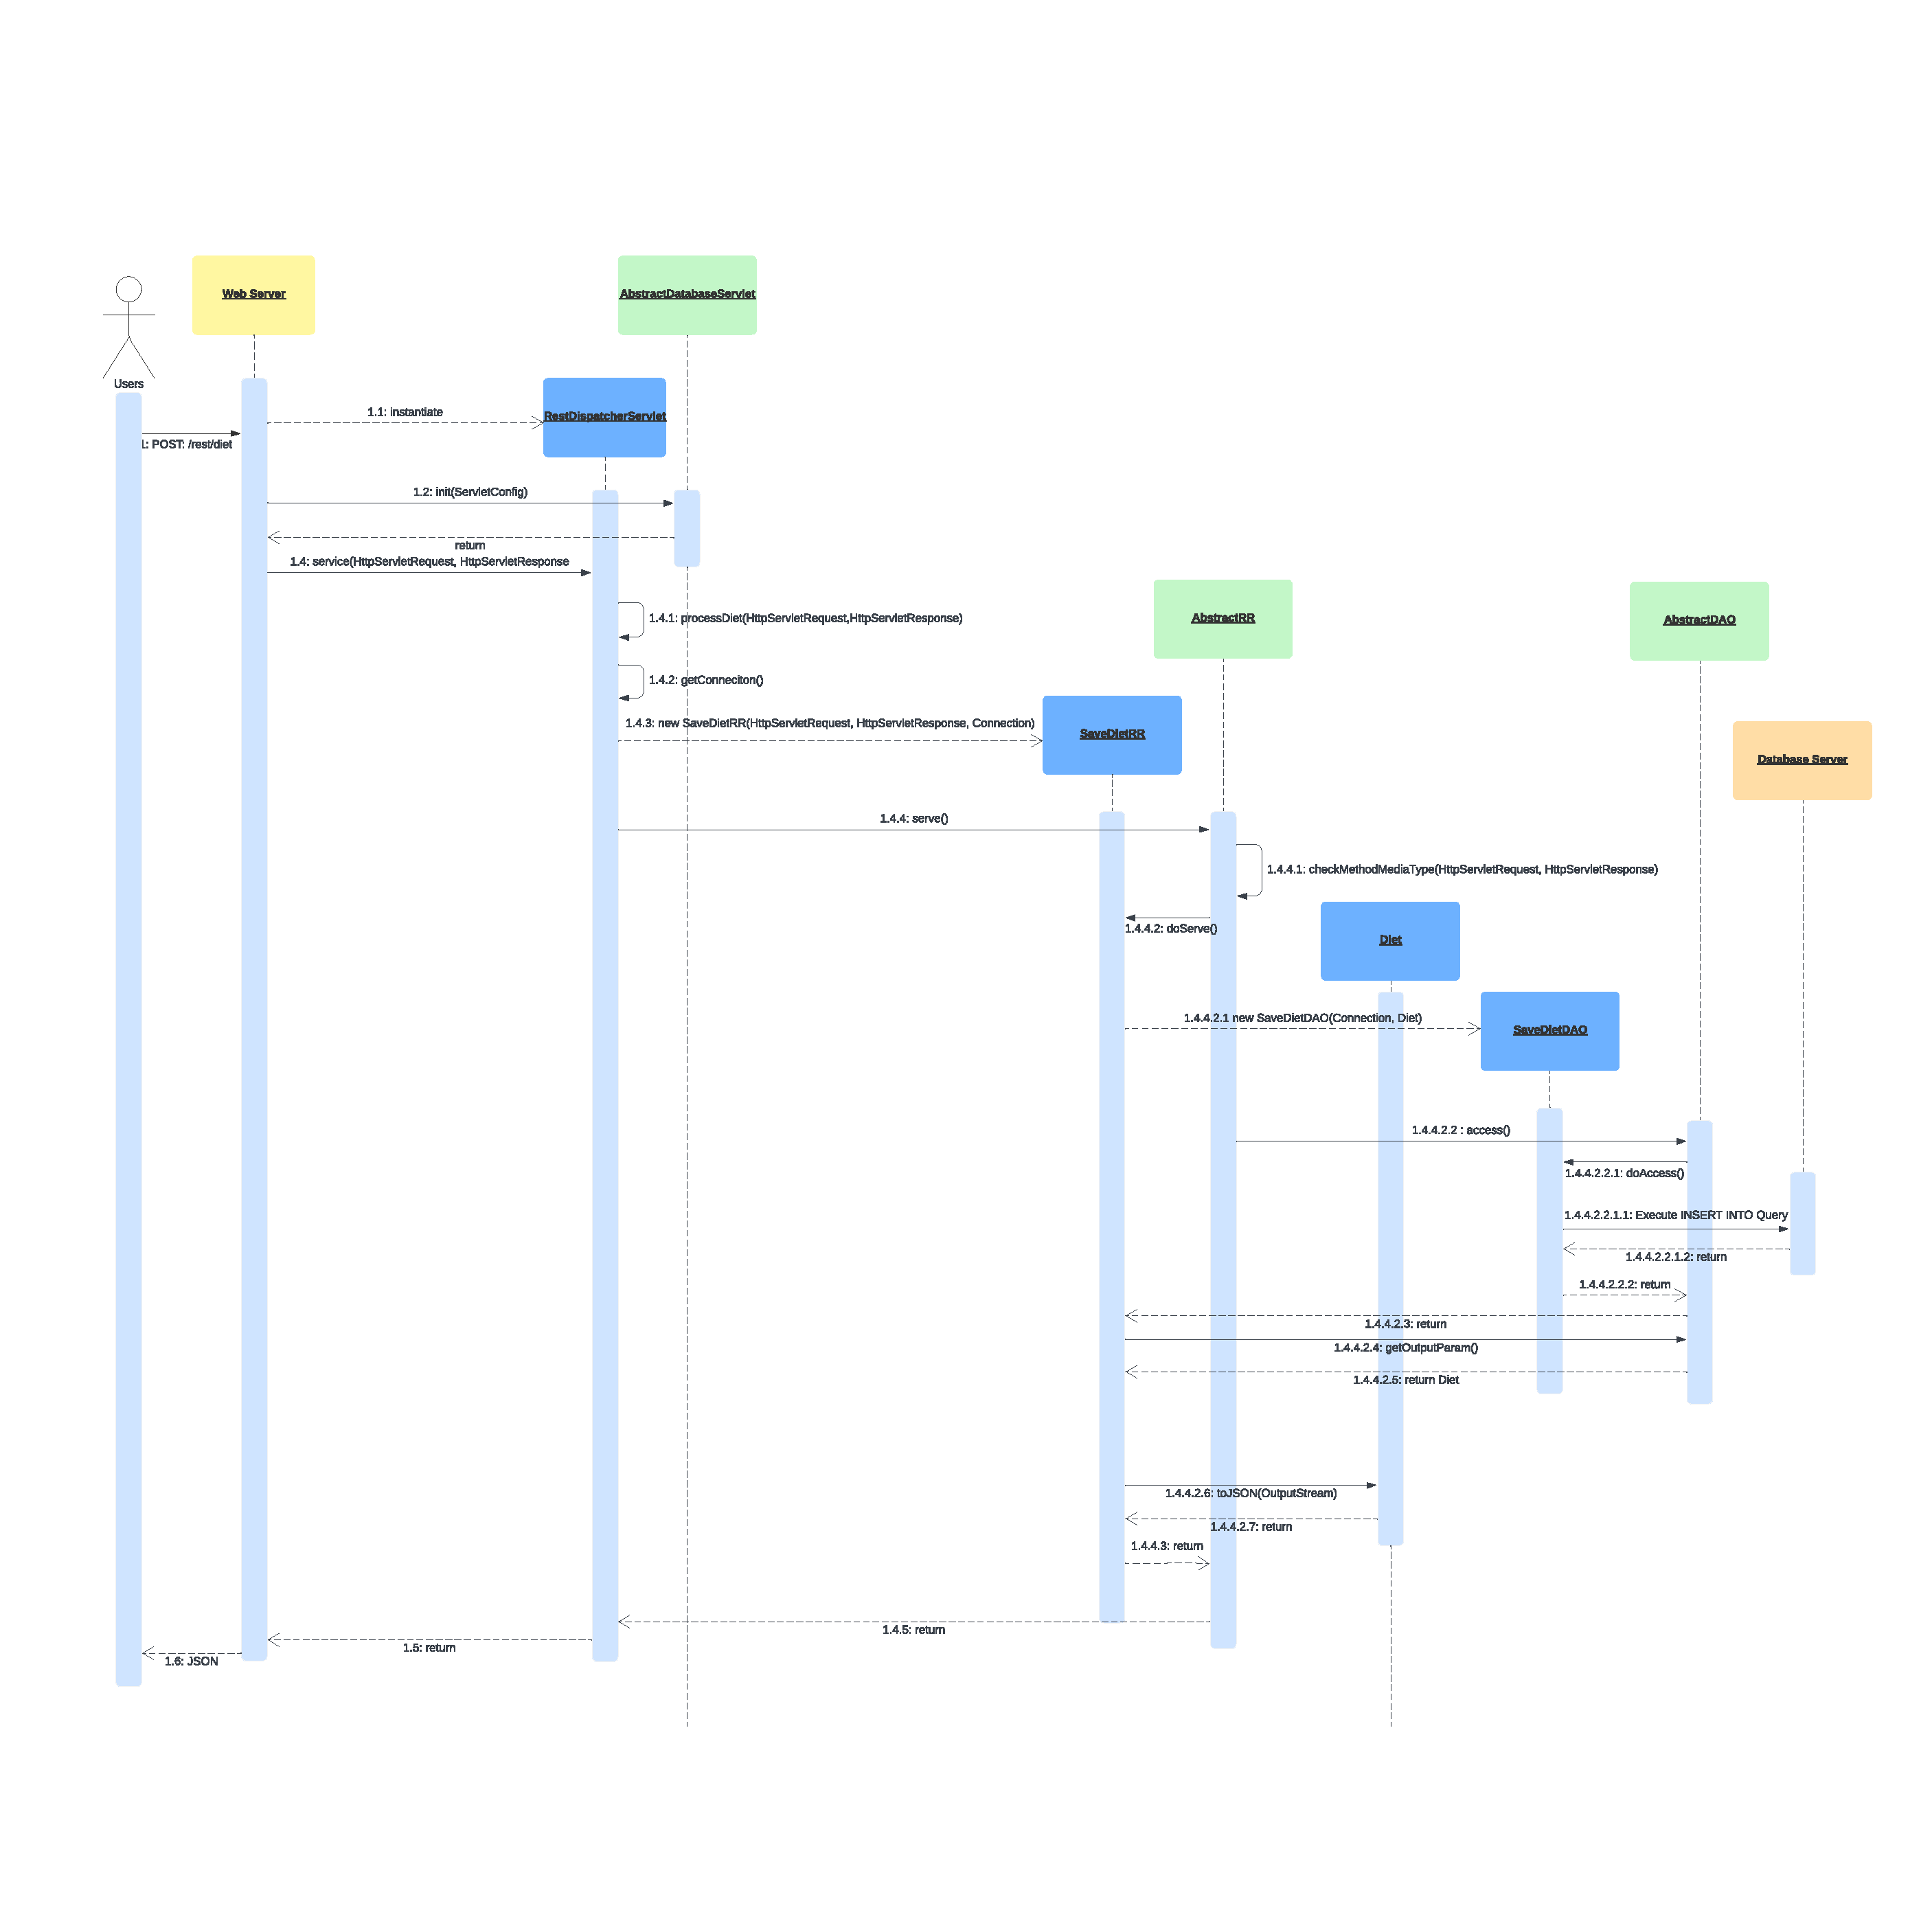
\includegraphics[scale=0.38]{Resources/SeqDiagPostDiet.pdf}
\textbf{Description}: 
In the schema above is shown the sequence diagram for the saving a diet operation.
The user sends a \textit{POST} request to the web server, specifying the URI /rest/diet and the diet in the body of the request. The web server calls the \textit{RestDispatcherServlet}, which calls the right service. The service (in this case DietService) analyzes and parses the URI and calls the right Rest Resources (in this case SaveDietRR). The resource create a new object of class \textit{Diet}, with the parameters passed in input.  After doing this, the resource instantiate a new object of the class \textit{SaveDietDAO}, which extends \textit{AbstractDAO} connecting to the database using the doAccess() method. After the connection is correctly established, the DAO executes the \textit{SQL} query and the diet is added to the database.
